\documentclass[../main.tex]{subfiles}
%!TEX root = ./analysisThrusterShaft.tex
\graphicspath {{../}}

\begin{document}
\subsection{Thruster Shaft} \label{thrustShaft}

\begin{figure}[H]
	\centering
	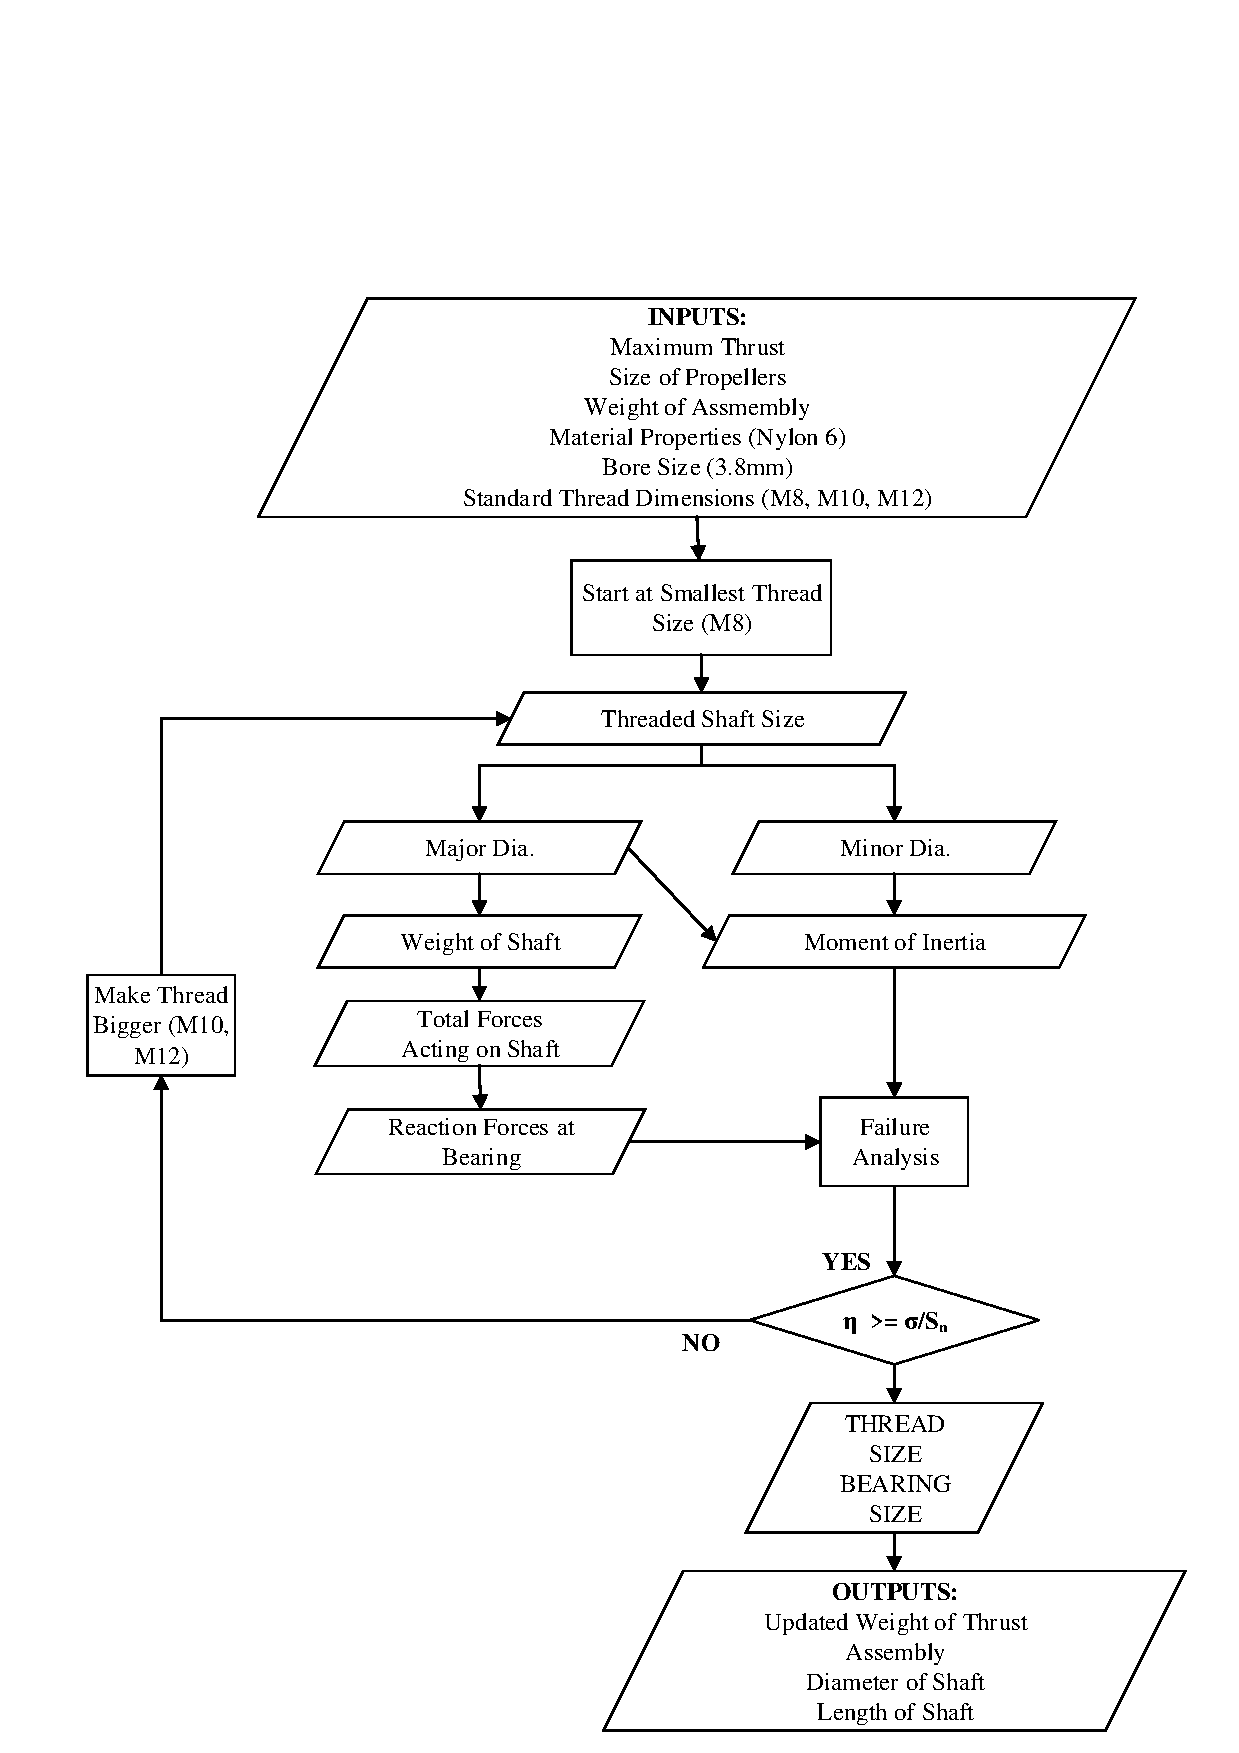
\includegraphics[width=.9\linewidth]{img/paramaterization/thrusterShaft.pdf}
	\caption{Parametrization Outline for the Thruster Shaft}
	\label{fig:ThrusterShaftParametrization}
\end{figure}

The thruster shaft analysis will optimize the diameter of the thruster shaft based on standard threaded shaft dimensions The Analysis will output the diameter of the shaft, the thread of the shaft, the length of the shaft, the weight of the shaft from which it updates the weight and centre of gravity of the entire thruster assembly. The inputs required for the analysis are the maximum thrust, the size of propellers, the weight of the assembly, the material properties of Nylon 6 REF?? (the shaft material), the bore size of the shaft which is 3.8[mm] and the standard thread dimensions from M8 to M16 REF ??.\\

The material nylon 6 was chosen because of its suitable strength, ease of manufacturability and weight. Aluminium was also considered but would have resulted in an over engineered component or a un-proportionally small radius while still being heavier. Results that justify this decision are shown at the end of the section REF??. The bore diameter of 3.8[mm] is based on the screw that attaches the shaft axially to the thrust vectoring motor, shown in FIG ??.\\

The scenario for the analysis is that descried in Loading Scenario, Section \ref{loadingScenarios}, Maximum Downward Force show in FIG??? where all forces are with reference to the coordinate system $XYZ$ defined by the pitch of the airship. The shaft is analysed in simple bending where it is cantilevered at the bearing in the thrust vector motor assembly shown in figure ???. The analysis begins by calculating the required length of shaft for the propeller size, as well as the position of the propeller with reference to the bearing. Following the the forceSolver REF??? code is used to solve the force and moments at the bearing that are resisting the weight of the shaft and motor/propeller assembly as well as the thrust force. Because in this scenario both the thrust and the weight are acting in the same direction all forces are acting in the x direction. So the greatest stress will be generated by the moment about z. Stress is calculated using the equation \ref{eqn:thrustShaftStress} shown below, assuming that the maximum stress will occur when the shaft is in tension at the upper outer edge. 
\begin{equation}
\label{eqn:thrustShaftStress} 
\sigma _{Shaft}  = \dfrac{M_{z}c}{I} 
\end{equation}
since it is a hollow cylinder the distance to the centroid $c$ in this equation is simply the minor radius of the shaft $r_{minor}$. The moment of inertia about z for a hollow cylinder is described by equation \ref{eqn:hollowInertia} below.
\begin{equation}
\label{eqn:hollowInertia} 
I _{z}  = \dfrac{\pi}{4} (r_{minor}^4 - r_{bore}^4)
\end{equation}

This stress is then used to determine the safety factor by Brittle Mohr-Coulomb Theory \cite[227]{shigley}.

\begin{equation}
\eta = \dfrac{S_{ut}}{\sigma _a} \Rightarrow 3 \geq \dfrac{S_{ut}}{\sigma _a}
\end{equation}

Due to the medium failure likelihood a safety factor $\eta$ of 3 is used. If for the shaft diameter used does not meet this requirement, the code selects the next highest standard threaded shaft diameter and runs through the analysis using those numbers. This repeats until the safety factor is met. 
\end{document}